\section{字典排列法}

\title[第2讲\quad 字典排列法]{第2讲\quad 字典排列法} 
\author{}
\date{}
\begin{frame}
    \titlepage
\end{frame}

\begin{frame}
    \frametitle{课前测}
    \begin{figure}[H]
        \centering 
    \end{figure}
\end{frame}

\begin{frame}
    \frametitle{知识梳理}
\end{frame}

\begin{frame}
    \frametitle{MISSION 1}
    \textit{同学们,在进行字典排列法时,我们应当如何做到不重不漏呢?}
\end{frame}

\begin{frame}
    \frametitle{探索1}
    \textit{(1)用数字1、2、3可以组成多少个不同的无重复数字的两位数?}
\end{frame}

\begin{frame}
    \frametitle{探索1}
    \textit{(2)用数字1、3、6可以组成多少个不同的无重复数字的三位数?}
\end{frame}

\begin{frame}
    \frametitle{探索2}
    \textit{(1)用数字1、2、3可以组成多少个不同的两位数?}
\end{frame}

\begin{frame}
    \frametitle{探索2}
    \textit{(2)用数字1、3、6可以组成多少个不同的三位数?}
\end{frame}

\begin{frame}
    \frametitle{捉虫时刻}
    \begin{figure}[H] 
        \centering
        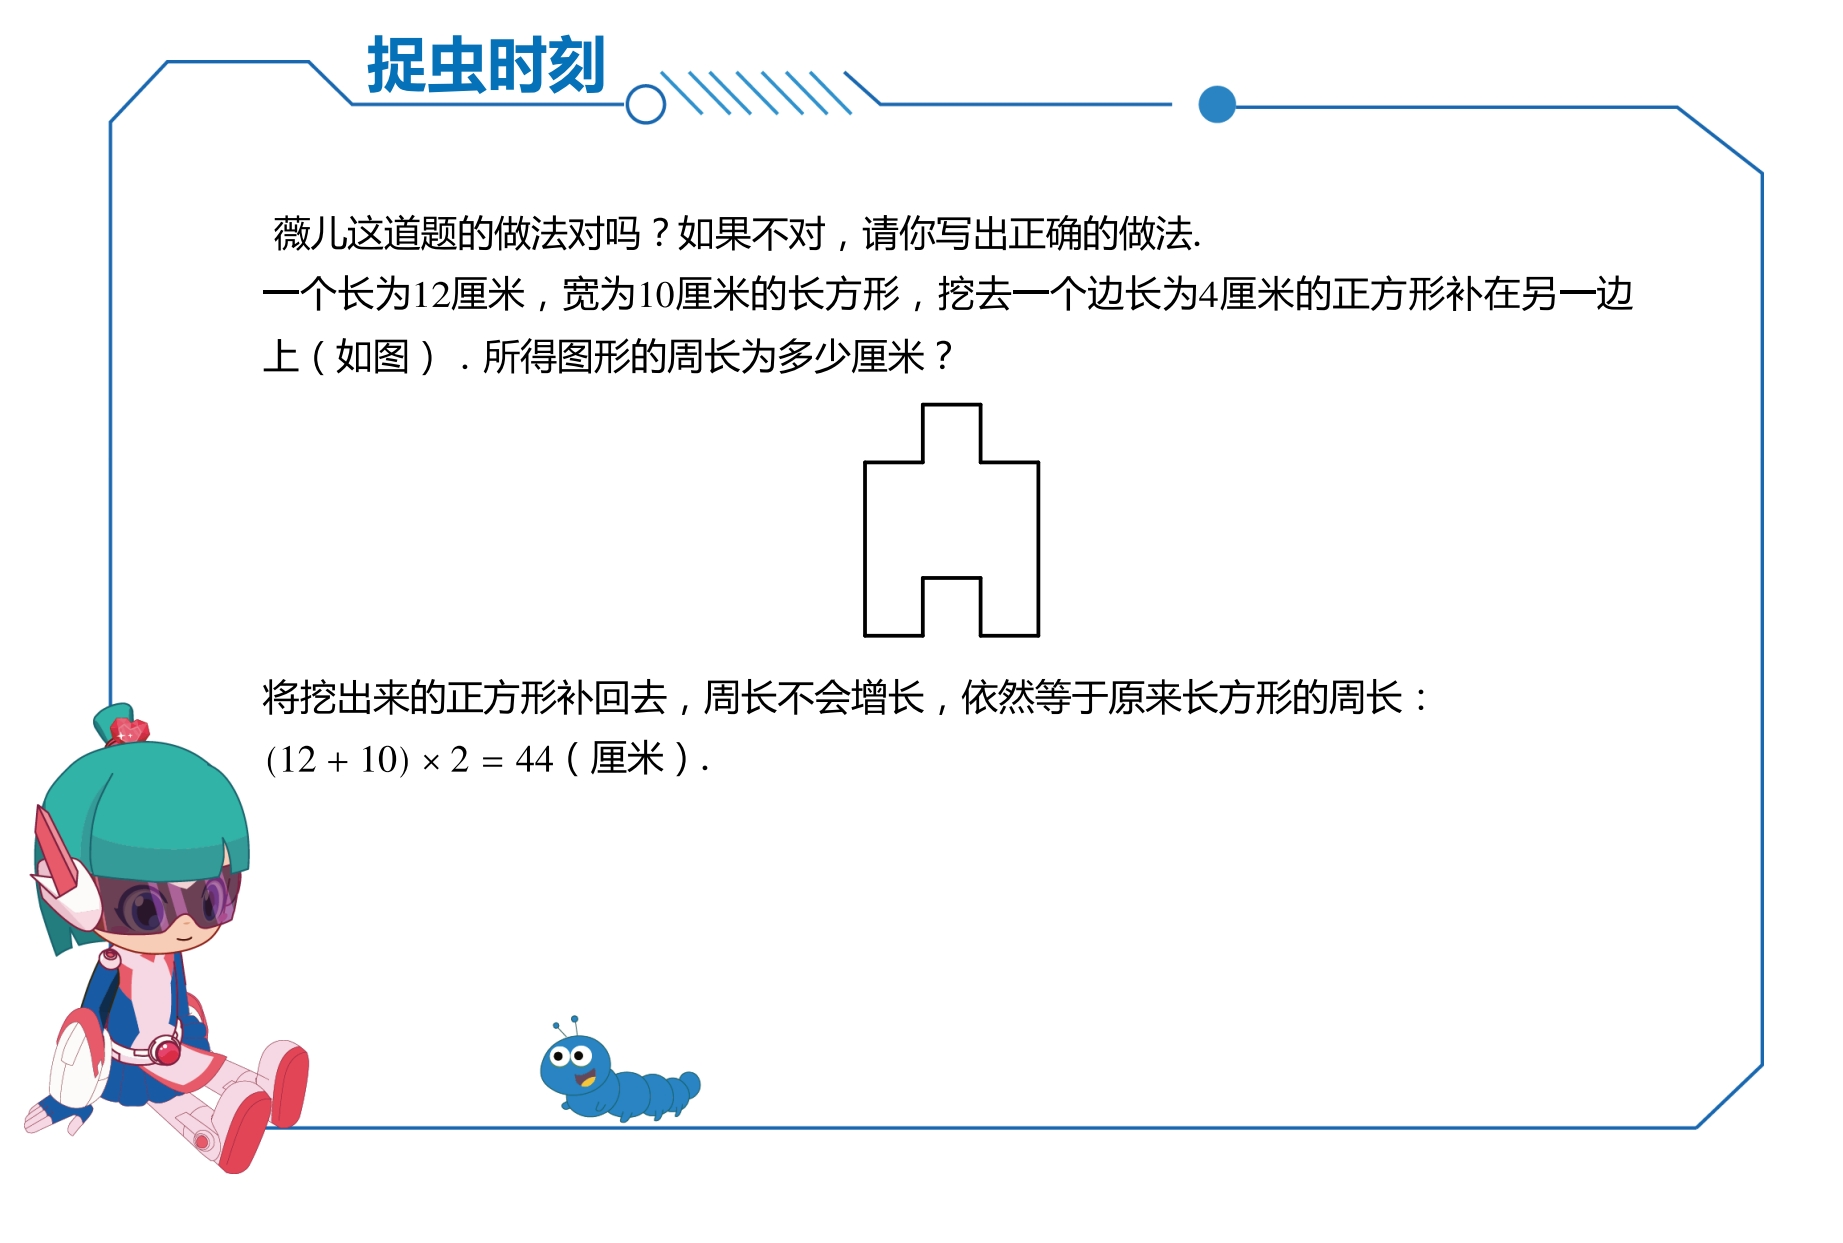
\includegraphics[width=1\textwidth]{./pics/Chapter_1/zhuochong1.png}
    \end{figure}
\end{frame}

\begin{frame}
    \frametitle{探索3}
    \textit{用数字1、2、3可以组成多少个不同的无重复数字的自然数?}
\end{frame}

\begin{frame}
    \frametitle{课堂互动}
    \begin{figure}[H] 
        \centering
        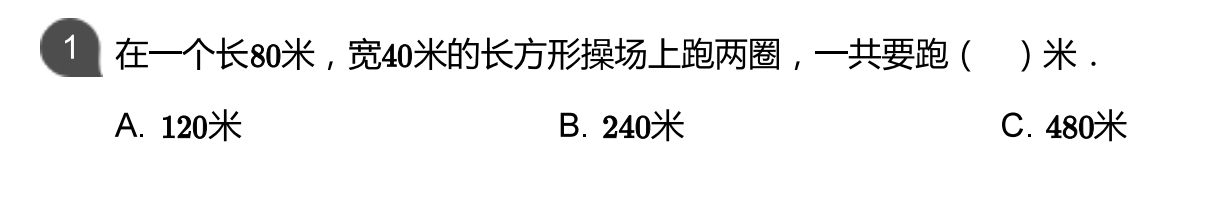
\includegraphics[width=1\textwidth]{./pics/Chapter_1/kthd1.png}
    \end{figure}
\end{frame}

\begin{frame}
    \frametitle{课堂互动}
    \begin{figure}[H] 
        \centering
        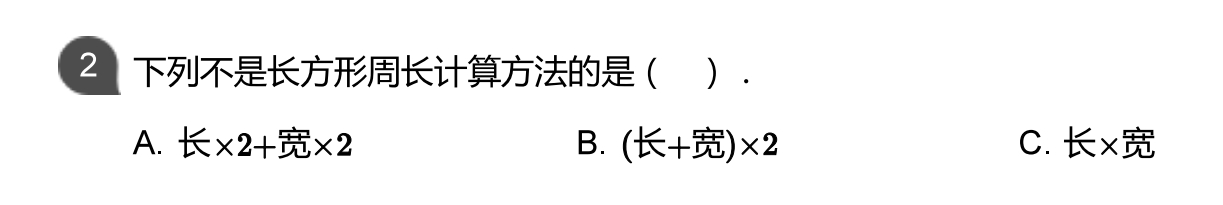
\includegraphics[width=1\textwidth]{./pics/Chapter_1/kthd2.png}
    \end{figure}
\end{frame}

\begin{frame}
    \frametitle{课堂互动}
    \begin{figure}[H] 
        \centering
        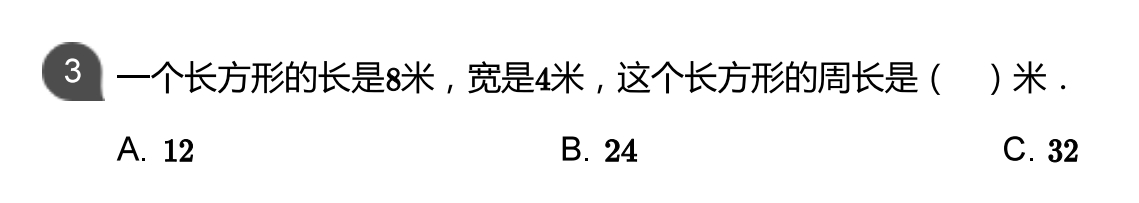
\includegraphics[width=1\textwidth]{./pics/Chapter_1/kthd3.png}
    \end{figure}
\end{frame}

\begin{frame}
    \frametitle{MISSION 2}
    \textit{在无序问题中,我们应当如何进行枚举?}
\end{frame}

\begin{frame}
    \frametitle{探索4}
    \textit{艾迪与薇儿做游戏,在分别标有1到10的10个完全一样的小球中,艾迪任意取出2个小球(不计取出顺序),由薇儿计算两球所标的数之和,若和大于10,则薇儿获胜.那么能使薇儿获胜的小球取法共有多少种?}
\end{frame}

\begin{frame}
    \frametitle{铺垫2}
    \textit{如图,把一个大正方形分割成9个小正方形,这9个小正方形的周长之和是72厘米,原来大正方的周长是厘米?}
    \begin{figure}[H] 
        \centering
        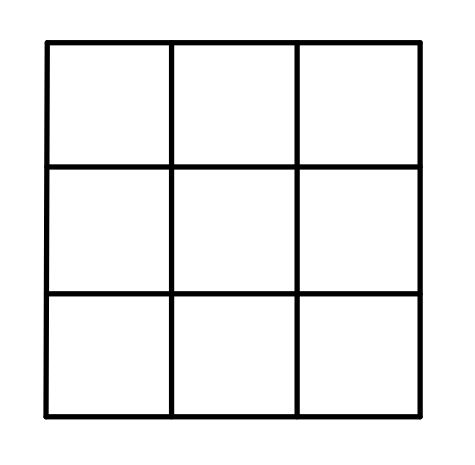
\includegraphics[width=0.5\textwidth]{./pics/Chapter_1/pudian2.png}
    \end{figure}
\end{frame}

\begin{frame}
    \frametitle{探索5}
    \textit{艾迪去儿童餐厅买15元特惠套餐,他有若干张1元、2元、5元的纸币,但是购买特惠套餐的条件是必须找出一共有多少种不同的付钱方法(要求每种纸币都有),眼看优惠时间就要截止了,同学们你能帮助艾迪顺利买到优惠套餐吗 ?}
\end{frame}

\begin{frame}
    \frametitle{铺垫3}
    \textit{把12个边长是1厘米的正方形纸拼成长方形.第( )种拼法拼成的图形周长最短}
    \begin{figure}[H] 
        \centering
        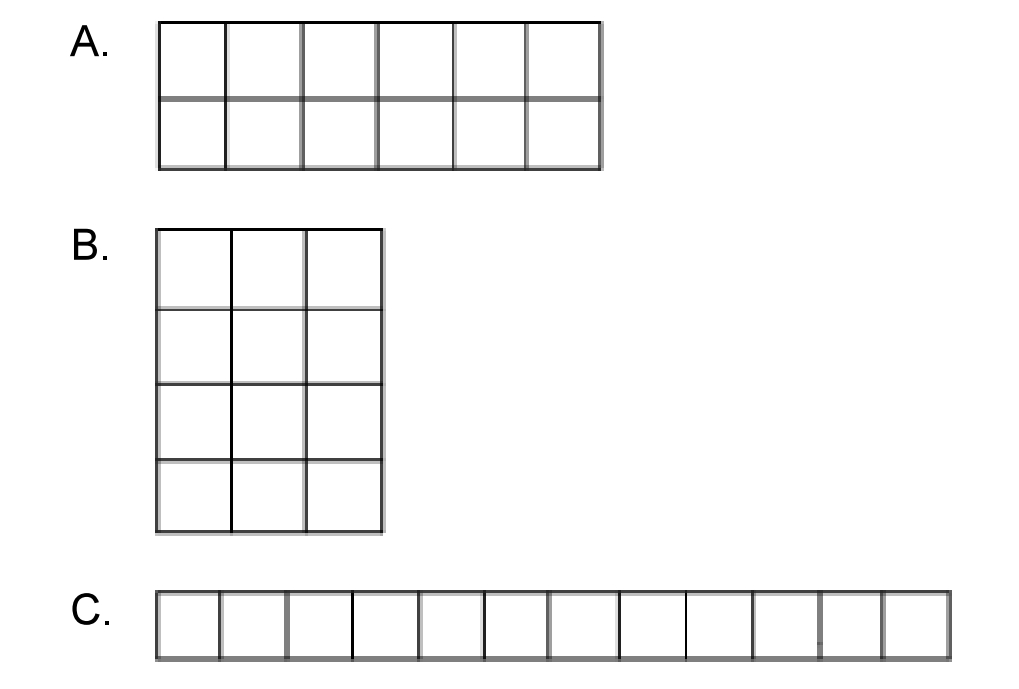
\includegraphics[width=1\textwidth]{./pics/Chapter_1/pudian3.png}
    \end{figure}
\end{frame}

\begin{frame}
    \frametitle{探索6}
    \textit{在某地有四种不同面值的硬币,如图所示,假若你恰有这四种硬币各1枚。问:共能组成多少种不同的钱数?}
\end{frame}

\begin{frame}
    \frametitle{探索7}
    \textit{博士给艾迪与薇儿上课,课上介绍了“拐弯”的概念. } \\
    \textit{博士:``对于一行数,,如果有三个数abc依次排一起,且a >b,c>b或者a<b,c<b,我们就称它发生了一次拐弯.'' \\
    艾迪:``我懂了,比如4321没有拐弯,像1243就发生了一次拐弯.'' \\
    薇儿:``没错,再比如1324就发生了两次拐弯.'' \\
    博士:``非常棒!看来你们都掌握得非常扎实了,现在我要考考你们了,如果我们将1,2,3,4排成一行,则能使这行数刚好发生两次拐弯的排列方法共有多少种.''}
\end{frame}

\begin{frame}
    \frametitle{铺垫4}
    \textit{一个长方形被分成了9小块,其中4块周长已经标出,则大长方形的周长为
    多少厘米}
    \begin{figure}[H] 
        \centering
        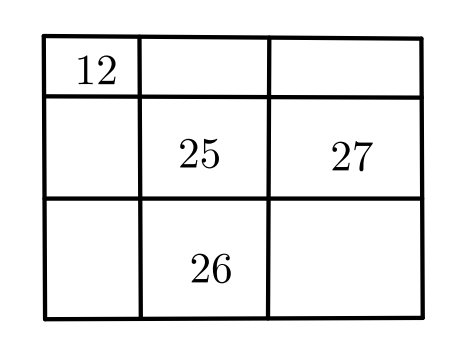
\includegraphics[width=0.5\textwidth]{./pics/Chapter_1/pudian4.png}
    \end{figure}
\end{frame}

\begin{frame}
    \frametitle{探索8}
    \textit{一次,齐王与田忌赛马,每人各有等级不同的4匹马,这8匹马按照从快到慢的排序分别是齐王的一等马,田忌的一等马,齐王的二等马,田忌的二等马,齐王的三等马,田忌的三等马,齐王的四等马,田忌的四等马.田忌已经提前知道齐王本次赛马的出场顺序是一等、二等、三等、四等,他可以安排种不同的出场顺序,才能保证自己至少战平齐王呢?同学们,你们能帮田忌找出所有可能的决策吗 ?}
\end{frame}
